% ||||||||||||||||||||||||||||||
% |||||| 3.2 Quintessence ||||||
% ||||||||||||||||||||||||||||||


% ------------------------------------------------
% labels: \label{[type]:cosmo:quintessence:[name]}
% ------------------------------------------------








The general picture interprets scalar-field theories as a group of scalar--tensor theories; a subgroup of modifications to gravity in which a scalar field is added to the total action. By going through all possible covariants with maximum second order time derivatives in four dimensional spacetime, one arrives at the most general formulation of these types of theories, the \emph{Hordenski theory}. Said theory is summed up by the total Lagrangian density $\mathcal{L}\nped{H} = \mathcal{L}\ped{m} + M\nped{Pl}^2 \sum_{i=2}^{5} \mathcal{L}_i$, where $\mathcal{L}_i$ are built up by derivatives of the scalar field, the Einstein tensor and arbitrary functionals of the scalar field $\phi$ and its kinetic term $X = - \frac{1}{2} \phi\^{;\mu}\phi\_{;\mu}$.%
\footnote{%
With the usual notation convention and arbitrary functionals $G_i$, the Lagrangian densities $\mathcal{L}_i$ are given by the following:
\begin{equation*}
    \begin{split}
        \mathcal{L}_2 &= G_2(\phi, X), \\
        \mathcal{L}_3 &= G_3 (\phi, X)\sq \phi, \\
        \mathcal{L}_4 &= G_4 (\phi, X)\mathcal{R} + G_{4,X}(\phi, X) \pclosed{ {(\sq \phi)}^2 - \phi\_{;\mu\nu} \phi\^{;\mu\nu}}, \\
        \mathcal{L}_5 &= G_5 \mathcal{G}\_{\mu\nu}\phi\^{;\mu\nu} - \sfrac{1}{6} G_{5,X}(\phi, X)  \pclosed{ {(\sq \phi)}^3 + 
        2\phi\indices{^\nu_{;\mu}}\phi\indices{^\mu_{;\nu}} - 3  \phi\_{;\mu\nu} \phi\^{;\mu\nu} \sq \phi},
    \end{split}
\end{equation*}%
where $G_{i,X}= \pdv*{G_i}{X}$.
}~%
Let $\mathcal{L}_i=0$ as a starting point. %
General relativity---represented by the Einstein--Hilbert action---is retrieved with $\mathcal{L}_4 = \mathcal{R}/2$.  By also setting $\mathcal{L}_2 = X(\phi)-V(\phi)$, we get a quintessence model. Performing relevant variations eventually gives an equation of motion that is indistinguishable from standard GR with $\mathcal{L}\ped{m} \to \mathcal{L}\ped{m} + \mathcal{L}_2$ in the stress--energy tensor on the right-hand side of the Einstein equation. Thus, quintessence models are not actually modified gravity theories, but adds to the total matter in the universe, and should be classified as a scalar-field theory rather than a scalar--tensor theory. %
% \citep{christiansenCosmologicalSimulationsPhase2024}. 





\subsection{General framework}\label{sec:cosmo:quintessence:framework}
    \comment{Softer start}
    We go through the dynamics of a scalar field $\phi$ that is associated with a kinetic term $X=- \frac{1}{2} g\^{\mu\nu} \phi\_{;\mu}\phi\_{,\nu}$ and potential energy $V(\phi)$ in broad terms. This will lay the foundation for our treatment of the (a)symmetron model in~\cref{sec:cosmo:quintessence:asymmetron}.


    % \deleteme{
    %     We argued in~\cref{sec:GR:diffgeo:conformal} that \checkthis{observables are preserved under conformal transformations of the metric.} \comment{Short text about Jordan and Einstein frames, conformal duality?}  
    % }

    % In the Jordan frame, matter fields---denoted collectively by $\Psi$---couple minimally to gravity. In the Einstein frame where the Einstein--Hilbert action assumes its usual form, matter may couple non-minimally to the scalar $\phi$
    The dynamics of the bosonic field $\phi$ is described by the Einstein-frame (see~\cref{sec:GR:diffgeo:conformal}) action% \comment{fix}
    \begin{equation}\label{eq:cosmo:quintessence:quintessence_action_Einstein}
        S =\integ[4]{x\sqrt{-g}} \cclosed{ \frac{M\nped{Pl}^2}{2} \mathcal{R} + X(\phi) - V(\phi)} + S\ped{(m)}[\widetilde{g}\_{\mu\nu} , \Psi],
    \end{equation} 
    where $\Psi$ collects all matter fields, which couple minimally to the Jordan-frame metric,
    \begin{equation}
        \widetilde{g}\_{\mu\nu} = A^2 (\phi) g\_{\mu\nu}% = A^2(\phi) \cdot  a^2(\tau) \eta_{\mu\nu},
    \end{equation}
    and $S\ped{(m)}$ is the total matter action. 
    Without the presence of this last term, the equation of motion for the scalar field is $\sq \phi = V_{,\phi}$. %
    % \nc{Some article}[appendix?] shows that 
    The minimal coupling to matter contributes such that~$\sq\phi \supset - A^{3} A_{,\phi}\widetilde{T}\ped{(m)}$, where $\widetilde{T}\ped{(m)}= {}\ap{(m)}\widetilde{T}\_{\mu\nu}\widetilde{g}\^{\mu\nu}$ is the trace of the Jordan-frame matter SE tensor~\citep{hinterbichlerSymmetronCosmology2011,christiansenAsevolutionRelativisticNbody2023}. In particular, 
    \begin{equation}
        \sq\phi = V_{,\phi}(\phi) - A^{3}(\phi) A_{,\phi}(\phi)\widetilde{T}_m.%\ped{(m)}.
    \end{equation}
    We model the matter content as non-interacting, perfect fluids indexed $s$ with equation-of-state parameter $w_s$ such that the trace becomes $\widetilde{T}\ped{(m)}\rvert\ped{p.f.} = \sum_s (3w_s-1 )\widetilde{\rho}_s$.  
    % The equation of motion for $\phi$ reads
    % \begin{equation}
    %     \sq \phi = {V\ped{eff}}_{,\phi},%; \quad V\ped{eff}(\phi) \equiv V(\phi) - A^3(\phi) A_{,\phi}(\phi) \widetilde{T}\ped{m},
    % \end{equation}
    % where 
    % \begin{align}
    %     V\ped{eff}(\phi) &\equiv V(\phi) - A^3(\phi) A_{,\phi}(\phi) \widetilde{T}\ped{m},\nonumber \\
    %     &= V(\phi)  - A^3(\phi) A_{,\phi}(\phi) \sum_{s} (1-3 w_s) \widetilde{\rho}_s 
    % % \end{align}
    % is the effective potential~\citep{hinterbichlerSymmetronCosmology2011}. 
    We have $\widetilde{\rho}_s\propto (Aa)^{-3(1+w_s)} \equiv A^{-3(1+w_s)}\rho_s$, where $\rho_s=a^{-3(1+w_s)}$ defines a scaled energy density, conserved in the Einstein frame, and $a$ is the Einstein-frame scale factor. Now
    \begin{equation}
        \sq \phi = V_{,\phi}(\phi) - A_{,\phi}(\phi) \sum_{s} A^{-3w_s}(\phi) (3w_s-1)\rho_s,
    \end{equation}
    which for near-constant $\rho_s$ reduces to $\sq \phi = V_{\mathrm{eff},\phi}$ where~\citep{hinterbichlerSymmetronCosmology2011}
    %dust-like matter $w_s\simeq 0$ reduce to 
    \begin{equation}
        V\ped{eff} = V(\phi) + \sum_s A^{1-3w_s}(\phi) \rho_s
    \end{equation}
    is the effective potential.%~\rcomment{Check if this is only symmetron.}. 

    % The minimal coupling to matter contributes such that~$\sq\phi \supset - A^{-1} A_{,\phi}T\ped{m} $, which amounts to writing
    % \begin{equation}
    %     \sq \phi = {V\ped{eff}}_{,\phi}; \quad V\ped{eff}(\phi) \equiv V(\phi) - \ln{A(\phi)} \cdot T\ped{m}.
    % \end{equation}
    % % Here, $T\ped{m}= g\^{\mu\nu}T\indices*{^{\mathrm{(m)}}_{\mu\nu}}$ 
    % Here, $T\ped{m}=A^4 \widetilde{T}\ped{m}$, $ \widetilde{T}\ped{m}=  {}\ap{(m)}\widetilde{T}\_{\mu\nu}\widetilde{g}\^{\mu\nu} $, is the trace of the Einstein-frame matter SE tensor. 
    % We model the matter content as non-interacting, perfect fluids indexed $s$ with equation-of-state parameter $w_s$ such that the trace becomes
    % \begin{equation}
    %     \widetilde{T}\ped{m}\rvert\ped{p.f.} = \sum_s (3w_s-1 )\widetilde{\rho}_s
    % \end{equation}
    
    % For a perfect fluid, $T\ped{m}\rvert\ped{p.f.}=-\rho + 3p$, and in the non-relativistic limit, we have $p\to 0$. %\speak{Maybe write ${}\ap{(m)}T\_{\mu\nu}$ etc.}

    % \paragraph{Fifth force.} %

    \subsubsection{Review}

    Matter particles in the Jordan frame obey the simple geodesic equation as there is no coupling to $\phi$. On the other hand, particles in the Einstein frame matter sector experience a \newconcept{fifth force} due to the universal coupling. The fifth-force concept captures the non-trivial right-hand side of in the geodesic equation,
    \begin{equation}\label{eq:cosmo:quintessence:framework:fifth_force}
        % \dv[2]{\vec{x}}{t} 
        \dv[2]{\vec{x}}{t} \supset \frac{\vec{F}_5}{m} = - \frac{\beta}{M\nped{Pl}} \vec{\nabla}\phi.
    \end{equation}
    Thus, 
    $\beta$ is 
    a measure of the strength of the fifth force relative to the Newtonian gravitational force.  
    % \comment{Violation of WEP. Maybe refer to equations in~\cref{sec:GR:einstein}?}

    % Matter particles in the Jordan frame move freely, i.e. obey the geodesic equation, whereas articles in the Einstein frame matter sector do not. 
    % \phpar[about screening mechanism?]

    % \paragraph{Screening.} %
    % \comment{Write short about screening mechanism!}
    % To 

    The dynamic, effective equation-of-state parameter is 
    \begin{equation}
        w_{(\phi)} =  \frac{p_{(\phi)}}{\rho_{(\phi)}}= \frac{\frac{1}{2a^2} \dot{\phi}^2 - V(\phi) }{\frac{1}{2a^2} \dot{\phi}^2 + V(\phi)},
    \end{equation}
    for which $\lim_{\dot{\phi}\to 0}{w_{(\phi)}}=w_\Lambda = -1$. %
    These models are thus often proposed in context of dark-energy models to explain the accelerated cosmic expansion. We will not consider this directly in this project.





    \subsection{Asymmetron model}\label{sec:cosmo:quintessence:asymmetron}
    The particular scalar-field model characterised by the symmetric Mexican-hat potential
    \begin{equation}
        V(\phi) = \frac{\lambda}{4} \phi^4  - \frac{\mu^2}{2} \phi^2 + V_0
    \end{equation}
    is called the \newconcept{symmetron} model~\citep{hinterbichlerSymmetronCosmology2011}. This theory is invariant under reflection, $\phi\to -\phi$.\footnote{
        See~\citet[\namecrefs{chap:GR}~11,~12,~20 \&~22]{peskinIntroductionQuantumField1995} or~\citet[\namecref{chap:GR}~7]{kolbEarlyUniverse1990} for discussion on quantum corrections.
    } %
    % a \nc{requirement from quantum theory.}[lost reference:(] (\iftime{Comment on this.}) %
    Not equally well-established is the generalisation of this model called the \newconcept{\emph{a}symmetron}~\citep{perivolaropoulosGravitationalTransitionsExplicitly2022}, in which the potential is given an additional cubic term, $V(\phi)\supset -\kappa\phi^3/3 $. Here, one of the domains is favoured over the other. 

    Now, why would we want this asymmetry in the first place? It complicates things by breaking the $\Zn$ symmetry of the symmetron, so the theory only holds approximately. However, this asymmetry can aid in overcoming the domain wall problem, manifest in the inevitable biased domain wall collapse. We mentioned this briefly in~\cref{sec:cosmo:defects:dws}. %
    We stress that introducing asymmetry in this way is different from energy bias in the sense that not only is the energy in the two domains different, but the expectation values for $\phi$ are shifted.

    \begin{figure}[h]
        \centering
        {\includegraphics[width=\linewidth]{Background/asymmetron_demo.pdf}}
        \caption{The evolution of the (a)symmetron effective potential in (dashed red) solid blue. \figpanel{Panel I}~The potential before SSB, \figpanel{panel II}~at SSB, and \figpanel{panels III--VI} after SSB, with diluting density.
        % \iftime{Add two balls.}
        % \figpanel{Panel I} shows before SSB, while \figpanel{panel II} is at SSB.
        }
        \label{fig:cosmo:quintessence:asymmetron_demo}
    \end{figure}

    The simplest (a)symmetron model has the quadratic coupling
    \begin{equation}
        A(\phi)  = 1 +\frac{1}{2} \pclosed{\frac{\phi}{M}}^2 + \mathscr{O}\Big( {(\phi/M)}^4 \Big).
    \end{equation}
    We consider the matter content to be dust-like, so that $\widetilde{T}\ped{(m)}\simeq -\widetilde{\rho}\ped{(m)}$. The effective potential is then given by~\citep{hinterbichlerSymmetronCosmology2011}%\lcomment{Mention $V\ped{eff}=V(\phi)+A(\phi)\rho$?}
    \boxedeq{eq:cosmo:quintessence:asymmetron_effective_potential}{
    V\ped{eff}(\phi) = \frac{\lambda}{4} \phi^4 - \frac{\kappa}{3}\phi^3 + \frac{\mu^2}{2}\pclosed{\frac{\rho\ped{(m)}}{\mu^2M^2}-1} \phi^2 + V_0,}
    %
    up to an irrelevant constant. %
    This potential becomes unstable when (or where) $\rho\ped{(m)}\leq \mu^2M^2\equiv \rho_\ast$, and the field rolls into either of the two vacua We call $\rho_\ast$ the \textit{critical density}. From the cosmological perspective, ignoring $\kappa$, we imagine an initially dense region in the universe where a scalar field oscillates slightly around zero. The energy density dilutes and eventually reaches the critical density ($\rho\ped{(m)}=\rho_\ast$), spontaneously breaking the $\Zn$ symmetry, and separates the scalar field into domains according to their sign at the time. A schematic of this evolution is shown in~\cref{fig:cosmo:quintessence:asymmetron_demo}. The potential barriers created at this \emph{phase transition} correspond to the topological solitons discussed in~\cref{sec:cosmo:defects:dws}; namely cosmic domain walls.
    %  The potential barriers created at this \emph{phase transition} \checkthis{represent topological defects}, e.g.~domain walls.

    % \begin{figure}[h]
    %     \floatbox[{\capbeside\thisfloatsetup{capbesideposition={left,top},capbesidewidth=4cm}}]{figure}[\FBwidth]
    %     {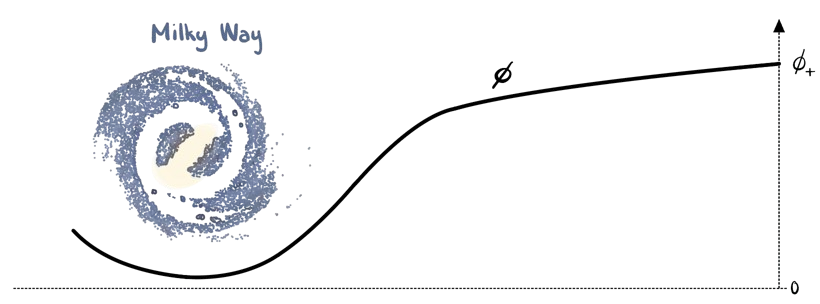
\includegraphics[width=5cm]{Background/symmetron_screen_milky.png}}
    %     {\caption{A test figure with its caption side by side}%\label{fig:test}}
    %     \label{fig:cosmo:quintessence:asymmetron_demo}
    % \end{figure}



    Let $\upsilon\equiv\rho\ped{(m)}/\rho_\ast = \rho\ped{(m)}/(\mu^2M^2)$. By setting $V\ped{eff,\phi}=0$, we find the vacuum expectation values (VEVs)
    \begin{equation}
        \phi_0 = 0 \quad \lor \quad \phi_\pm = \phi_\infty \pclosed{\bar{\kappa} \pm  \sqrt{\bar{\kappa}^2 +  1- \upsilon }},%\frac{\kappa \pm \sqrt{\kappa^2 + 4\lambda\mu^2 \pclosed{1- \rho\ped{m}/(\mu^2M^2)} } }{2\lambda}
    \end{equation}
    where we defined $\bar{\kappa} = \kappa / (2\mu \sqrt{\lambda}) $ and $\phi_\infty = \mu/\sqrt{\lambda}$. Note that the (real) VEV is zero before SSB for the symmetron ($\kappa=0$).
    % for the symmetron ($\kappa=0$), since the field is real,\comment{fix} VEV is zero before SSB. 
    We determine the stability of these minima by evaluating $V\ped{eff,\phi\phi}$ at $\phi=\phi_0,\phi_\pm$ and see that $\phi_0$ remains stable until $\rho\ped{(m)}=\rho_\ast$, and for $\rho\ped{(m)}\leq \rho_\ast$, $\phi_\pm$ are stable. % 
    % \footnote{This is not entirely true for the asymmetron, but we will not discuss this here.} %
    % We determine the stability of these vacua by evaluating $V\ped{eff,\phi\phi}$ at $\phi=\phi_0,\phi_\pm$ and see that $\phi_0$ remains stable until $\rho\ped{(m)}=\rho_\ast$.\footnote{This is not entirely true for the asymmetron, but we will not discuss this here.}


    \subsubsection{Screening}
    In this context, a \newconcept{screening mechanism} is a property of the model that removes the effect of the extra scalar field in the appropriate environment. The symmetron scalar field mediates fifth forces in low-density environments while being screened in dense regions. We illustrate this in~\cref{fig:cosmo:quintessence:symmetron_screen_milky}. 
    %  \blahblah

    \begin{figure}[h]
        \centering
        {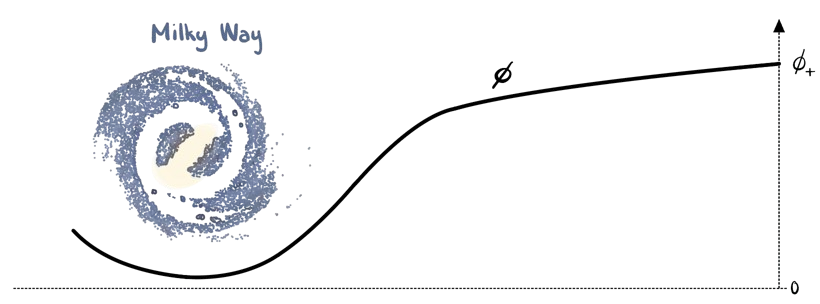
\includegraphics[width=\linewidth]{Background/symmetron_screen_milky.png}}
        {\caption{Schematic of the symmetron screening mechanism. It is clear that the vacuum expectation value goes to zero in dense regions. This example assumes a symmetron with Compton length scale $L\nped{C}\sim\mathscr{O}(\mathrm{kpc})$~\citep{burrageAccurateComputationScreening2024}. Illustration based on~\citet{christiansenCosmologicalSimulationsPhase2024}.}
        \label{fig:cosmo:quintessence:symmetron_screen_milky}}
    \end{figure}

    % \begin{bullets}
    %     \item Phase transition aspect
    %     \item Screening
    %     \item Comment on asymmetron
    % \end{bullets}

    \subsubsection{Free parameters}



    % \phpar[parameter space of asymmetron]

    The quartic coupling constant $\lambda$ measures the scalar self-interactions and $\mu$ defines the bare mass of the (a)symmetron. The cubic coupling $\kappa$ is a measure of the difference between the two vacua, and is zero in the symmetron case. The constant $V_0$ can be interpreted as a cosmological constant \textLambda~\citep{christiansenAsevolutionRelativisticNbody2023}, but we will not discuss this here. The conformal coupling scale $M$ governs the matter coupling strength~\citep{burrageAccurateComputationScreening2024}. We introduce the \newconcept{symmetron Compton wavelength}
    \begin{equation}\label{eq:cosmo:quintessence:symmetron_Compton_wavelength}
        L\nped{C} \equiv \frac{1}{\sqrt{2}\mu}
    \end{equation}
    which defines the range of the symmetron forces.\footnote{
        Note that some references consider the dynamical quantity $L\nped{C}\sqrt{1-\upsilon}$ to be the symmetron Compton wavelength, which is the actual dynamical range of the symmetron.
    } %
    Local tests of gravity require $M \lesssim 10^{-3} M\nped{Pl}$ for the quadratic coupling~\citep{burrageAccurateComputationScreening2024,hinterbichlerSymmetronCosmology2011,hinterbichlerScreeningLongRangeForces2010,hagalaCosmicTsunamisModified2017}. This is to say that fifth forces is mediated within a range $L\nped{C}\lesssim\mathrm{Mpc}$~\citep{hinterbichlerScreeningLongRangeForces2010}.

    % The 

    % \citet{burrageAccurateComputationScreening2024} sets the constraint $M \lesssim 10^{-3.6} M\nped{Pl}$ \blahblah

    








    








    